% Short version of ../slides.tex: the five timed slides cut to the minimum,
% the closing and backup slides unchanged. Five-minute talk: five timed slides (title, question, result, validation, lessons)
% followed by a closing slide and five backup slides (appendix), not timed. Build: ./build.sh
% Every number on the slides is copied from manuscript/numbers.tex,
% short-summary/comparison-numbers.tex or prompts/uso-de-tiempo-y-tokens.md;
% the two derived ones (+31%, 2.3x) are asserted in make_figures.py.
% The full five-minute version is ../slides.tex; the ten-minute one is ../v10min/.
\documentclass[aspectratio=169,11pt]{beamer}
\usetheme[progressbar=frametitle,numbering=fraction]{metropolis}
\usepackage{appendixnumberbeamer}
\usepackage[T1]{fontenc}
\usepackage[utf8]{inputenc}
\usepackage{lmodern}
\usepackage{amsmath}
\usepackage{mathtools}
\usepackage{graphicx}
\usepackage{tikz}
\usetikzlibrary{positioning,arrows.meta}
\graphicspath{{../figures/}}

\definecolor{ink}{HTML}{1F2937}
\definecolor{accent}{HTML}{1F5FA8}
\definecolor{warm}{HTML}{D9622B}
\definecolor{muted}{HTML}{6B7280}
\definecolor{paper}{HTML}{FFFFFF}
\setbeamercolor{normal text}{fg=ink,bg=paper}
\setbeamercolor{frametitle}{fg=white,bg=accent}
\setbeamercolor{progress bar}{fg=warm,bg=accent!30}
\setbeamercolor{alerted text}{fg=warm}
\setbeamerfont{frametitle}{size=\large}
\setbeamercolor{block body}{bg=accent!7}

\newcommand{\ext}{\mathsf{ext}}
\newcommand{\GB}{\mathsf{GB}}
\newcommand{\stat}[2]{{\large\bfseries\color{accent}#1\par}\vspace{1pt}{\scriptsize\color{muted}#2\par}}
\newcommand{\src}[1]{{\scriptsize\color{muted}#1}}
\newcommand{\hd}[1]{{\small\bfseries\color{accent}#1}}
\newcommand{\eqbox}[1]{%
  \begin{beamercolorbox}[wd=\linewidth,sep=4pt,center]{block body}#1\end{beamercolorbox}}

\title{Extremality shift of rotating black holes\\at finite Gauss--Bonnet coupling}
\subtitle{A research project carried out with AI agents}

\begin{document}

% ---------------------------------------------------------------- 1  title
\begin{frame}[plain]
\vspace*{0.8cm}
{\LARGE\bfseries\color{accent}Extremality shift of rotating black holes\\[2pt]
at finite Gauss--Bonnet coupling\par}
\vspace{0.3cm}
{\large A research project carried out with AI agents\par}
\vspace{0.7cm}
{\normalsize C.~Bejarano, D.~Blanco, A.~Goya, G.~Pérez-Nadal\par}
\vfill
{\footnotesize\color{muted}AI-Assisted Research course, FCEN--UBA \ \textperiodcentered{} \ 2 October 2026
\ \textperiodcentered{} \ \texttt{github.com/ddblanco/BHs}\par}
\end{frame}

% ---------------------------------------------------------------- 2  problem
\begin{frame}{The question}
\begin{columns}[c,onlytextwidth]
\column{.42\textwidth}\centering
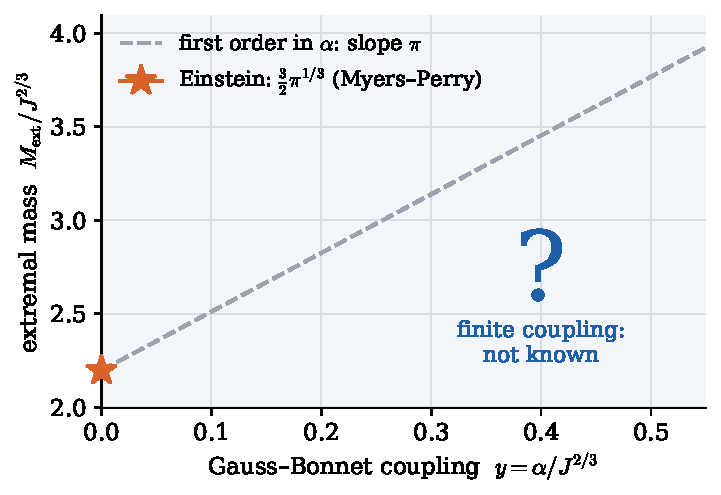
\includegraphics[width=.88\linewidth]{fig-question.pdf}\par\vspace{2pt}
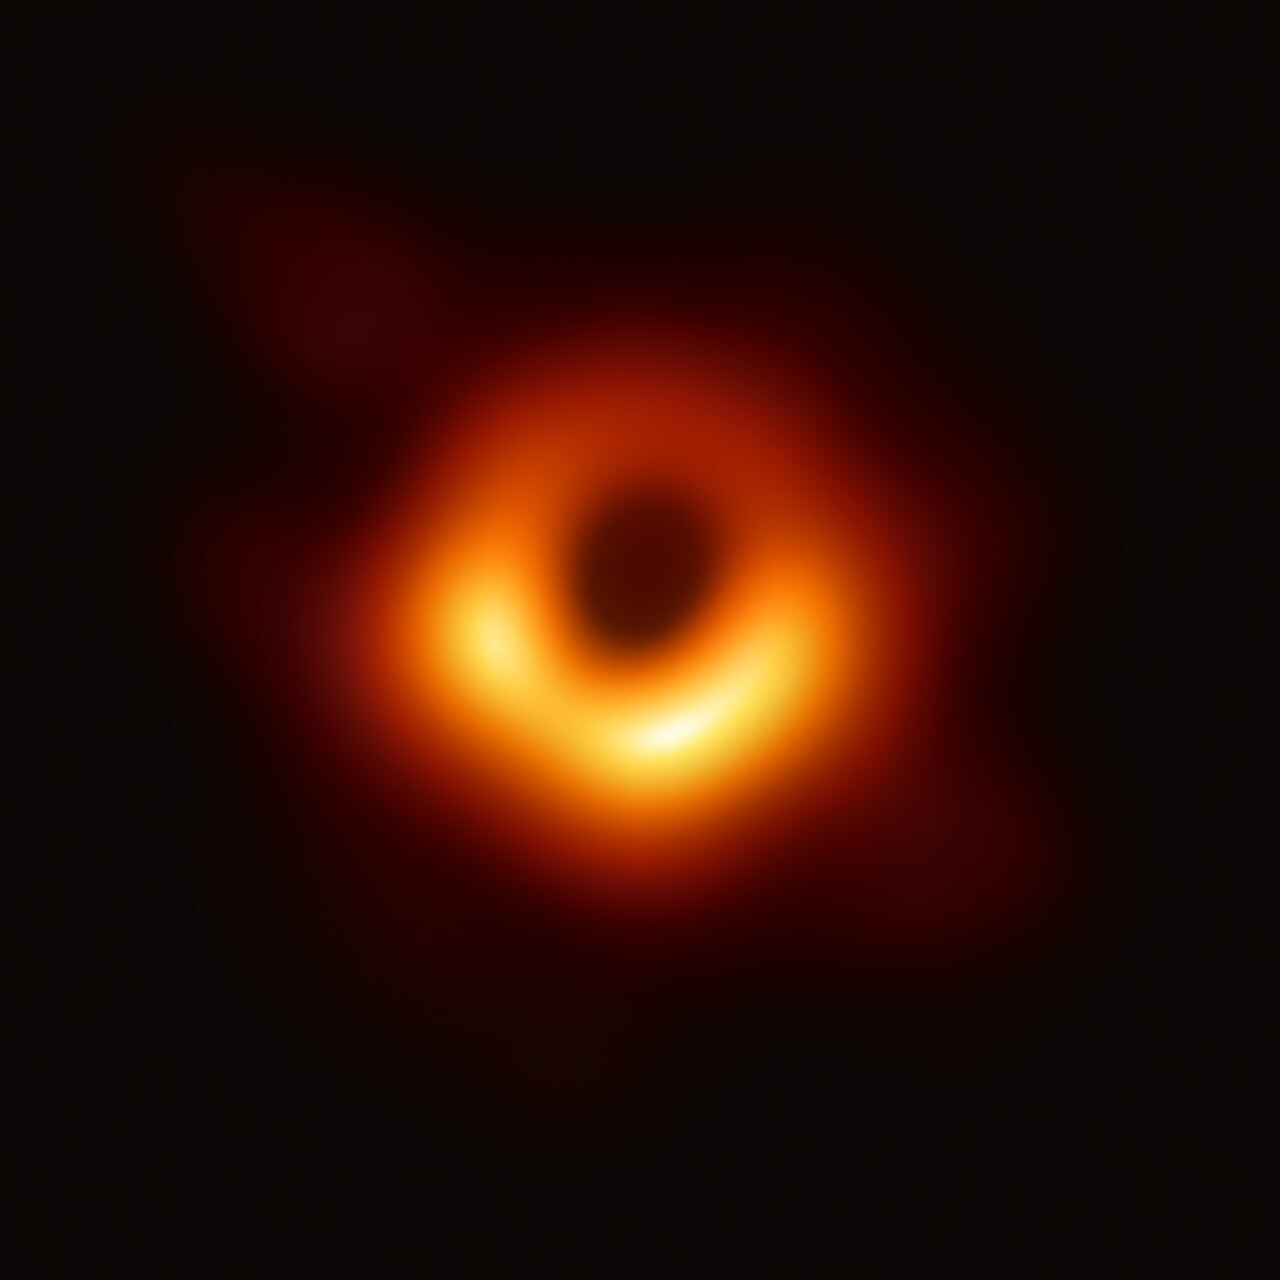
\includegraphics[width=.38\linewidth]{eht-photo.jpg}\par
\src{M87*, EHT (2019)}
\column{.54\textwidth}
\setlength{\abovedisplayskip}{2pt}\setlength{\belowdisplayskip}{10pt}
\hd{GR, 5D:} \ spin bound
\[M\ge\tfrac32\,\pi^{1/3}J^{2/3}\]
\hd{+ Gauss--Bonnet} \ $\alpha$:
\[M_\ext=\tfrac32\pi^{1/3}J^{2/3}+\pi\,\alpha+\mathcal O(\alpha^2)\]
\hd{Finite} $\alpha$\,?
\end{columns}
\end{frame}

% ---------------------------------------------------------------- 3  result
\begin{frame}{Result: the bound tightens, but not linearly}
\begin{columns}[c,onlytextwidth]
\column{.62\textwidth}\centering
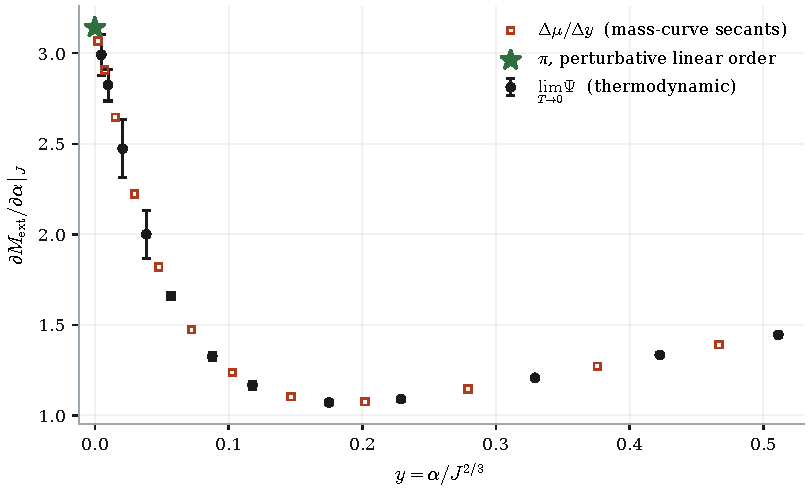
\includegraphics[width=\linewidth]{fig-shift.pdf}
\column{.34\textwidth}\centering
\[\frac{\partial M_\ext}{\partial\alpha}\bigg|_J=\alert{\Psi_\ext}\]
\vspace{10pt}
\stat{$>0$}{bound tightens}\vspace{10pt}
\stat{$\pi\!\to\!1.07\!\to\!1.44$}{not monotonic}
\end{columns}
\end{frame}

% ---------------------------------------------------------------- 4  validation
\begin{frame}{Validation}
\begin{columns}[c,onlytextwidth]
\column{.6\textwidth}\centering
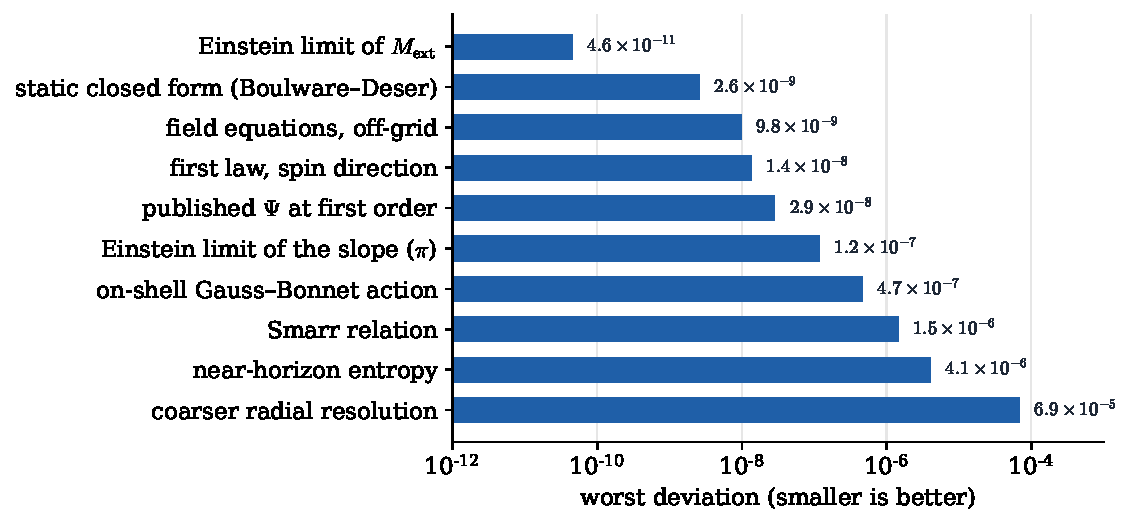
\includegraphics[width=\linewidth]{fig-checks.pdf}
\column{.36\textwidth}\small
\hd{Known solutions} reproduced\par\vspace{12pt}
\hd{Two independent routes} to $\Psi$ agree\par\vspace{12pt}
\hd{Main uncertainty:} $T\to0$ extrapolation
\end{columns}
\end{frame}

% ---------------------------------------------------------------- 5  experience
\begin{frame}{Working with agents}
\centering
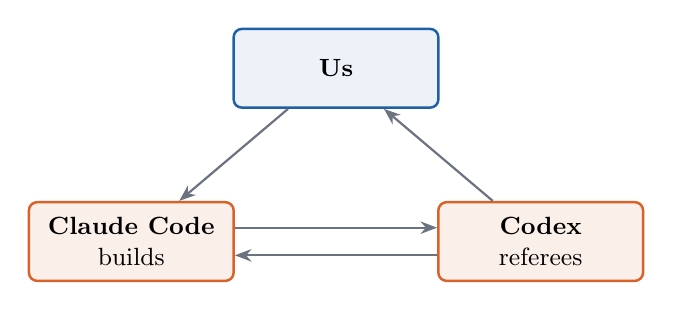
\begin{tikzpicture}[
  every node/.style={font=\small,align=center,rounded corners=3pt,
                     draw=accent,line width=0.9pt,fill=accent!8,minimum width=2.6cm,minimum height=1cm},
  hot/.style={draw=warm,fill=warm!10},
  >={Stealth[length=6pt]}]
\node (h) {\textbf{Us}};
\node[hot] (c) at (-2.6,-2.2) {\textbf{Claude Code}\\builds};
\node[hot] (x) at (2.6,-2.2) {\textbf{Codex}\\referees};
\draw[->,thick,muted] (h) -- (c);
\draw[->,thick,muted] ([yshift=5pt]c.east) -- ([yshift=5pt]x.west);
\draw[->,thick,muted] ([yshift=-5pt]x.west) -- ([yshift=-5pt]c.east);
\draw[->,thick,muted] (x) -- (h);
\end{tikzpicture}

\vfill
\large The cost is not writing code, it is \alert{verifying} it.
\vfill
\end{frame}

% ================================================================ after the talk
% \appendix here so that the frame total counts only slides 1-5.
\appendix

% ---------------------------------------------------------------- 6  thanks
\begin{frame}[standout]
Thank you for your attention\\[14pt]
{\normalsize\mdseries Matías and Nahuel, thanks for the AI course}
\end{frame}

% ================================================================ backup

% ---------------------------------------------------------------- A1
\begin{frame}{A1 \textperiodcentered{} Numerical method: solving the field equations}
\vspace{-6pt}
\begin{columns}[T,onlytextwidth]
\column{.53\textwidth}\scriptsize
\setlength{\abovedisplayskip}{1pt}\setlength{\belowdisplayskip}{1pt}
{\bfseries\color{accent}Equal-spin ansatz} $\Rightarrow$ ODEs in $r$ for $b,f,h,w$:
\[\begin{aligned}ds^2={}&-b\,dt^2+\frac{dr^2}{f}+r^2\bigl[d\theta^2+\sin^2\!\theta\cos^2\!\theta\,(d\varphi_1-d\varphi_2)^2\bigr]\\
&+h\,\bigl[\sin^2\!\theta\,d\varphi_1+\cos^2\!\theta\,d\varphi_2-w\,dt\bigr]^2\end{aligned}\]
horizon: $b=f=0$, $w=\Omega_H$;\ \ infinity: $b,f,h/r^2\to1$, $w\to0$\par
\column{.45\textwidth}\scriptsize
{\bfseries\color{accent}Discretise:} $\chi=1-r_H/r$, Chebyshev--Lobatto, $N=64$:
$R_N(u;\alpha,r_H,\Omega_H)=0$ \ ($4N$ eqs.)\\[2pt]
{\bfseries\color{accent}Solve:} damped Newton; continuation from Myers--Perry\\[2pt]
{\bfseries\color{accent}Accept:} $G_{\mu\nu}+\alpha H_{\mu\nu}<10^{-8}$ at 51 off-grid points\\[2pt]
{\bfseries\color{accent}Read off:} $b\simeq1+U/r^2$, $w\simeq W/r^4$ $\Rightarrow$ $M=-\tfrac{3\pi}8U$, $J=\tfrac\pi4W$
\end{columns}
\vspace{4pt}
\begin{columns}[T,onlytextwidth]
\column{.43\textwidth}\centering
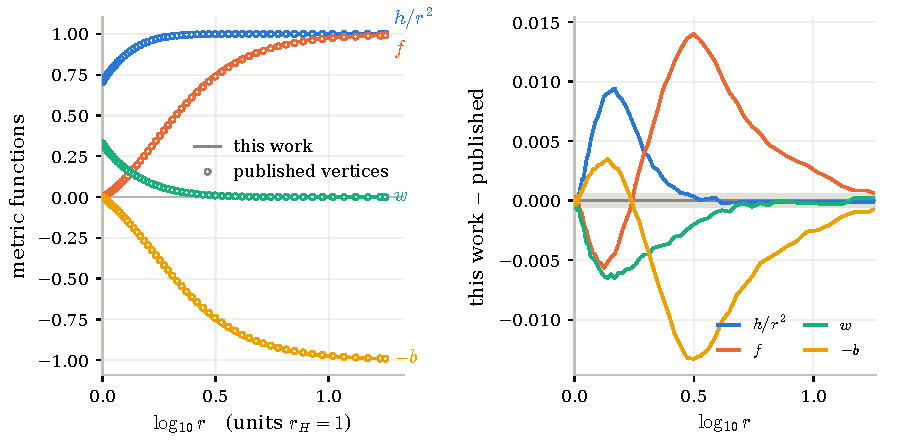
\includegraphics[height=3.6cm,trim=0 0 217bp 0,clip]{fig-paper-comparison.pdf}
\column{.55\textwidth}\centering
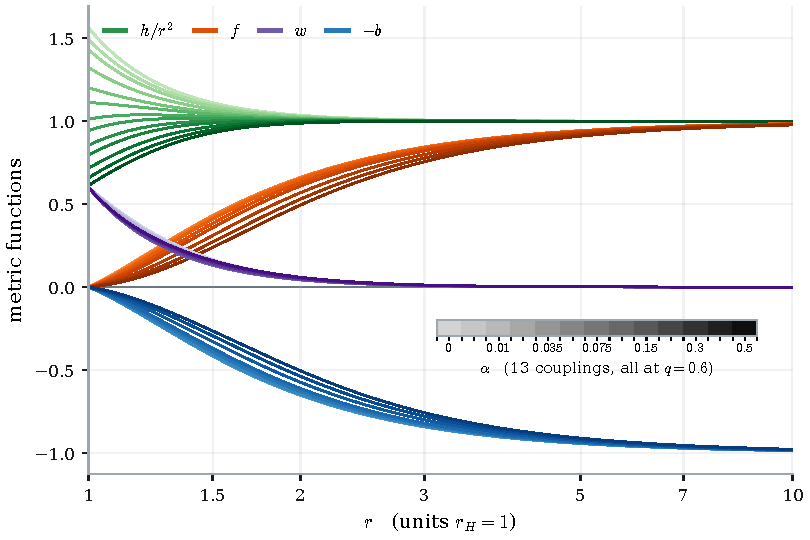
\includegraphics[height=3.6cm]{fig-profiles.pdf}
\end{columns}
\end{frame}

% ---------------------------------------------------------------- A2
\begin{frame}{A2 \textperiodcentered{} Numerical method: measuring $\Psi$ and reaching $T=0$}
\begin{columns}[T,onlytextwidth]
\column{.47\textwidth}\small
\hd{$\Psi$ from derivatives at fixed $(r_H,\Omega_H)$}
\[\Psi=\left.\frac{\partial M}{\partial\alpha}\right|_{S,J}=M_\alpha-T\,S_\alpha-2\Omega_H\,J_\alpha\]

\hd{Derivatives without finite differences}
\[\underbrace{\frac{\partial R_N}{\partial u}}_{\mathclap{\text{Newton Jacobian}}}\frac{du}{d\alpha}=-\frac{\partial R_N}{\partial\alpha}\]
\scriptsize one linear solve, no step size (implicit function theorem)

\medskip\small
\hd{Get cold, then extrapolate}\\
cubic fit through the 6 coldest states;\\
coldest $TJ^{1/3}\approx3\times10^{-6}$
\column{.51\textwidth}\centering
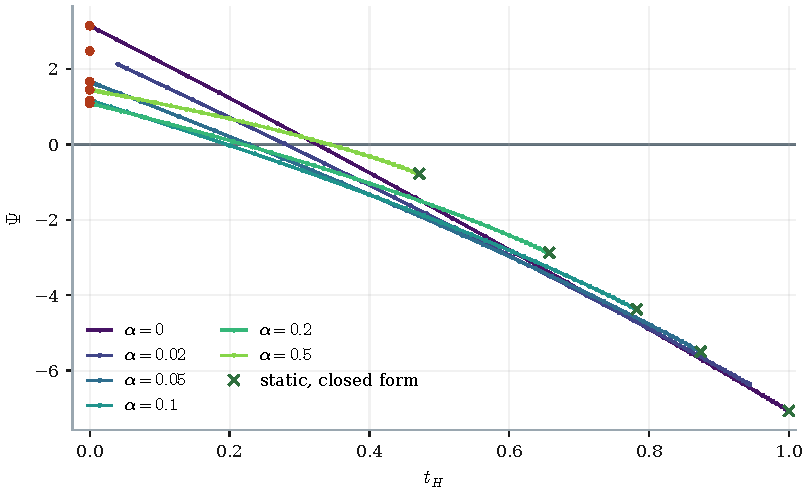
\includegraphics[width=\linewidth]{fig-potential.pdf}\\
\scriptsize $\Psi$ against temperature; red dots: the $T=0$ values (the slope)
\end{columns}
\end{frame}

% ---------------------------------------------------------------- A2b
% manuscript/main.tex, paragraphs "The potential from the Smarr relation" and
% "The potential as an on-shell action"; numbers from manuscript/numbers.tex.
\begin{frame}{A2b \textperiodcentered{} Two other routes to $\Psi$}
\begin{columns}[T,onlytextwidth]
\column{.48\textwidth}\small
\setlength{\abovedisplayskip}{3pt}\setlength{\belowdisplayskip}{3pt}
\hd{1. Smarr relation} \src{(scaling)}\\
weights: $M,\alpha\to2$, \ $S,J\to3$; Euler's theorem:
\[2M=3TS+6\Omega_HJ+2\alpha\Psi\]
\[\Rightarrow\quad\Psi=\frac{2M-3TS-6\Omega_HJ}{2\alpha}\]
\scriptsize charges of \alert{one} solution: no Jacobian, no derivative\\[2pt]
agrees to $1.45\times10^{-6}$ (313 states);\ useless as $\alpha\to0$
\column{.48\textwidth}\small
\setlength{\abovedisplayskip}{3pt}\setlength{\belowdisplayskip}{3pt}
\hd{2. On-shell Gauss--Bonnet action}\\
Gibbs potential = on-shell action per unit time; at fixed $(T,\Omega_H)$, $\alpha$ enters explicitly only through $\mathcal L_\GB$ (field equations remove the rest):
\[\Psi=-\frac1{16\pi}\int_\Sigma\!\sqrt{-g}\,\mathcal L_\GB\]
\scriptsize curvature of the solution only: no charge extraction either\\[2pt]
agrees to $4.67\times10^{-7}$ (43 states, away from extremality)
\end{columns}
\vfill
\centering\src{Both use the same numerical solutions; neither uses the linear solve of A2.}
\end{frame}

% ---------------------------------------------------------------- A3
\begin{frame}{A3 \textperiodcentered{} Physical meaning of the result}
\centering
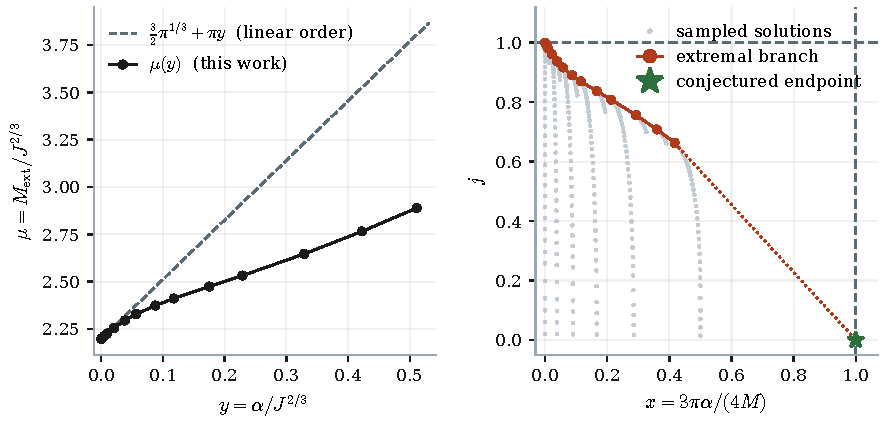
\includegraphics[width=.66\textwidth]{fig-massext.pdf}

\vspace{2pt}
\begin{columns}[T,onlytextwidth]
\column{.34\textwidth}\centering\small
\hd{Spin bound}\\
$\Psi_\ext>0\ \Leftrightarrow\ j_\ext$ falls:\\
less spin per unit mass
\column{.32\textwidth}\centering\small
\hd{Slope minimum}\\
$3\omega=\mu-y\,\mu'$\\
= fastest extremal horizon,\\ $\omega=\Omega_HJ^{1/3}$
\column{.34\textwidth}\centering\small
\hd{Why it rises again}\\
$M>\tfrac{3\pi}4\alpha$ \ forces\\
$\mu'\to\tfrac{3\pi}{4}\approx2.36$
\end{columns}
\end{frame}

% ---------------------------------------------------------------- A4
\begin{frame}[t]{A4 \textperiodcentered{} How it started: the first prompts}
\vspace{-4pt}
\begin{beamercolorbox}[wd=\linewidth,sep=4pt,leftskip=4pt]{block body}
\scriptsize\itshape ``El proyecto consiste en utilizar agentes de IA para implementar códigos
numéricos que permitan obtener soluciones de agujeros negros rotantes en
dimensión D>4 [\ldots] reproducir soluciones numéricas ya encontradas en la
literatura. [\ldots] el paso siguiente sería emprender la búsqueda de nuevas
soluciones.''\par\smallskip\upshape\tiny\color{muted}Prompt 1 --- 4 Sept, 19:16, to Codex
\quad\textperiodcentered{}\quad then ``Fijate que el proyecto realmente siga las indicaciones propuestas por el
docente del curso'' (3), ``ejecutar con subagentes'' (5), ``continuemos con el hito 3'', ``dale, avanzá''
\quad\textperiodcentered{}\quad \textbf{79} human prompts, 4--28 Sept \quad\textperiodcentered{}\quad Claude Code builds $\leftrightarrow$ Codex referees
\end{beamercolorbox}
\par\vspace{-16pt}\noindent
\begin{minipage}[t]{.44\textwidth}\vspace{0pt}\centering
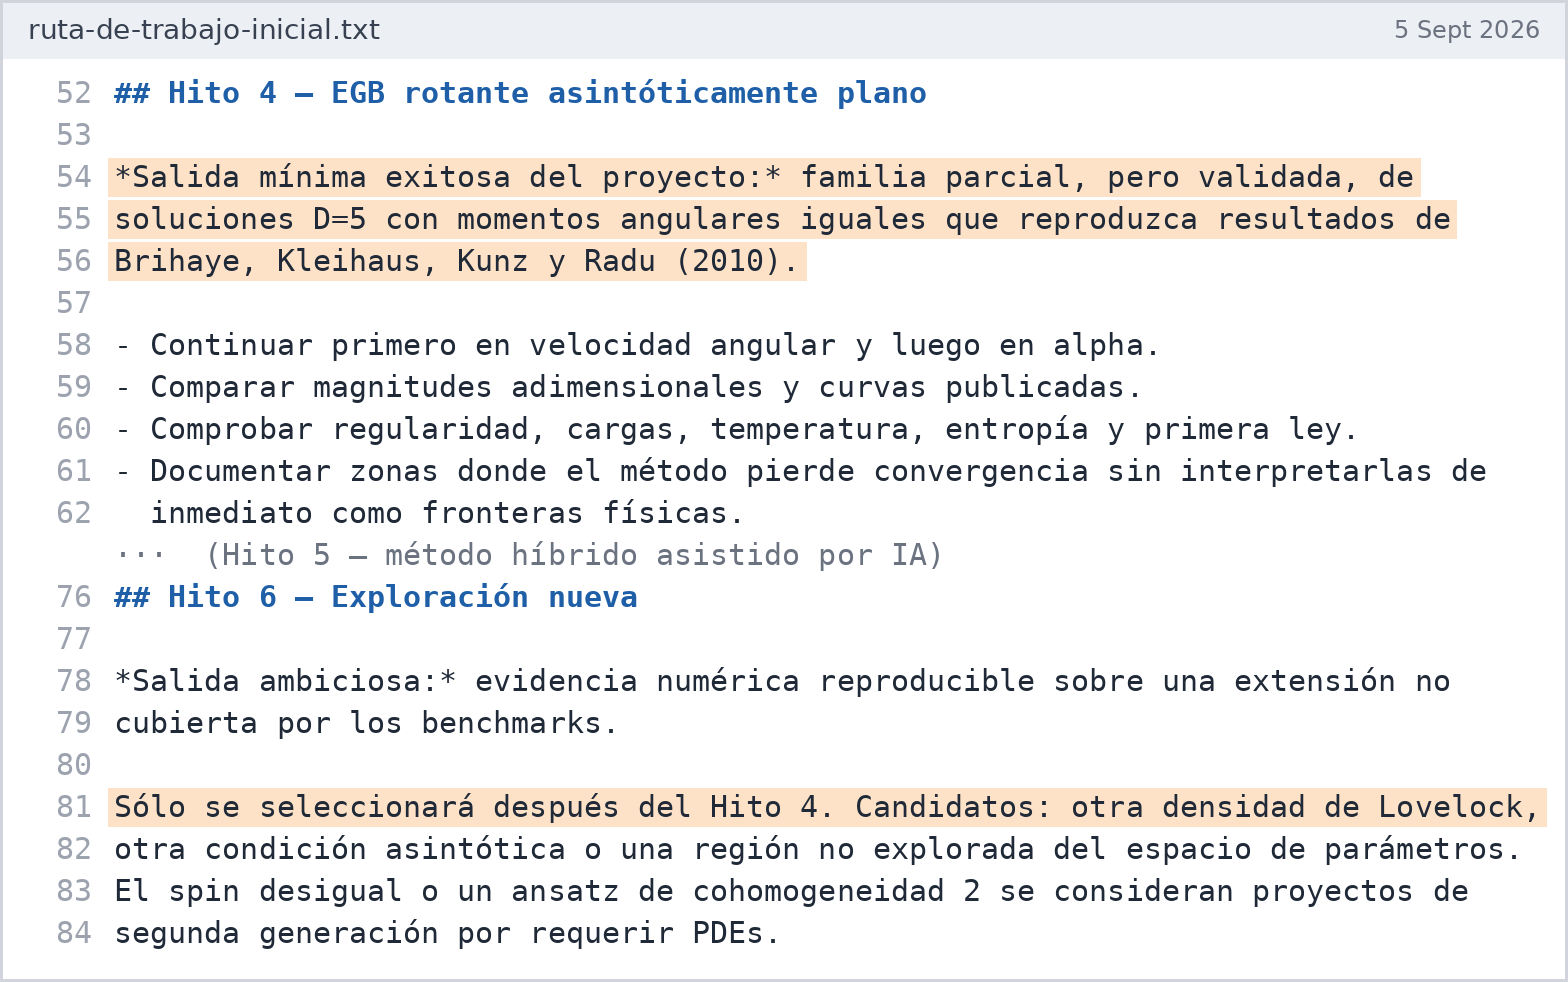
\includegraphics[width=.9\linewidth]{fig-roadmap.png}\par\vspace{2pt}
{\tiny\color{muted}first roadmap, 5 Sept. \textcolor{warm}{Hito 6} became $\Psi$;
Hito 8 ($T\to0$, paper, referees) was not in the plan.\par}
\end{minipage}\hfill
\begin{minipage}[t]{.52\textwidth}\vspace{0pt}\centering
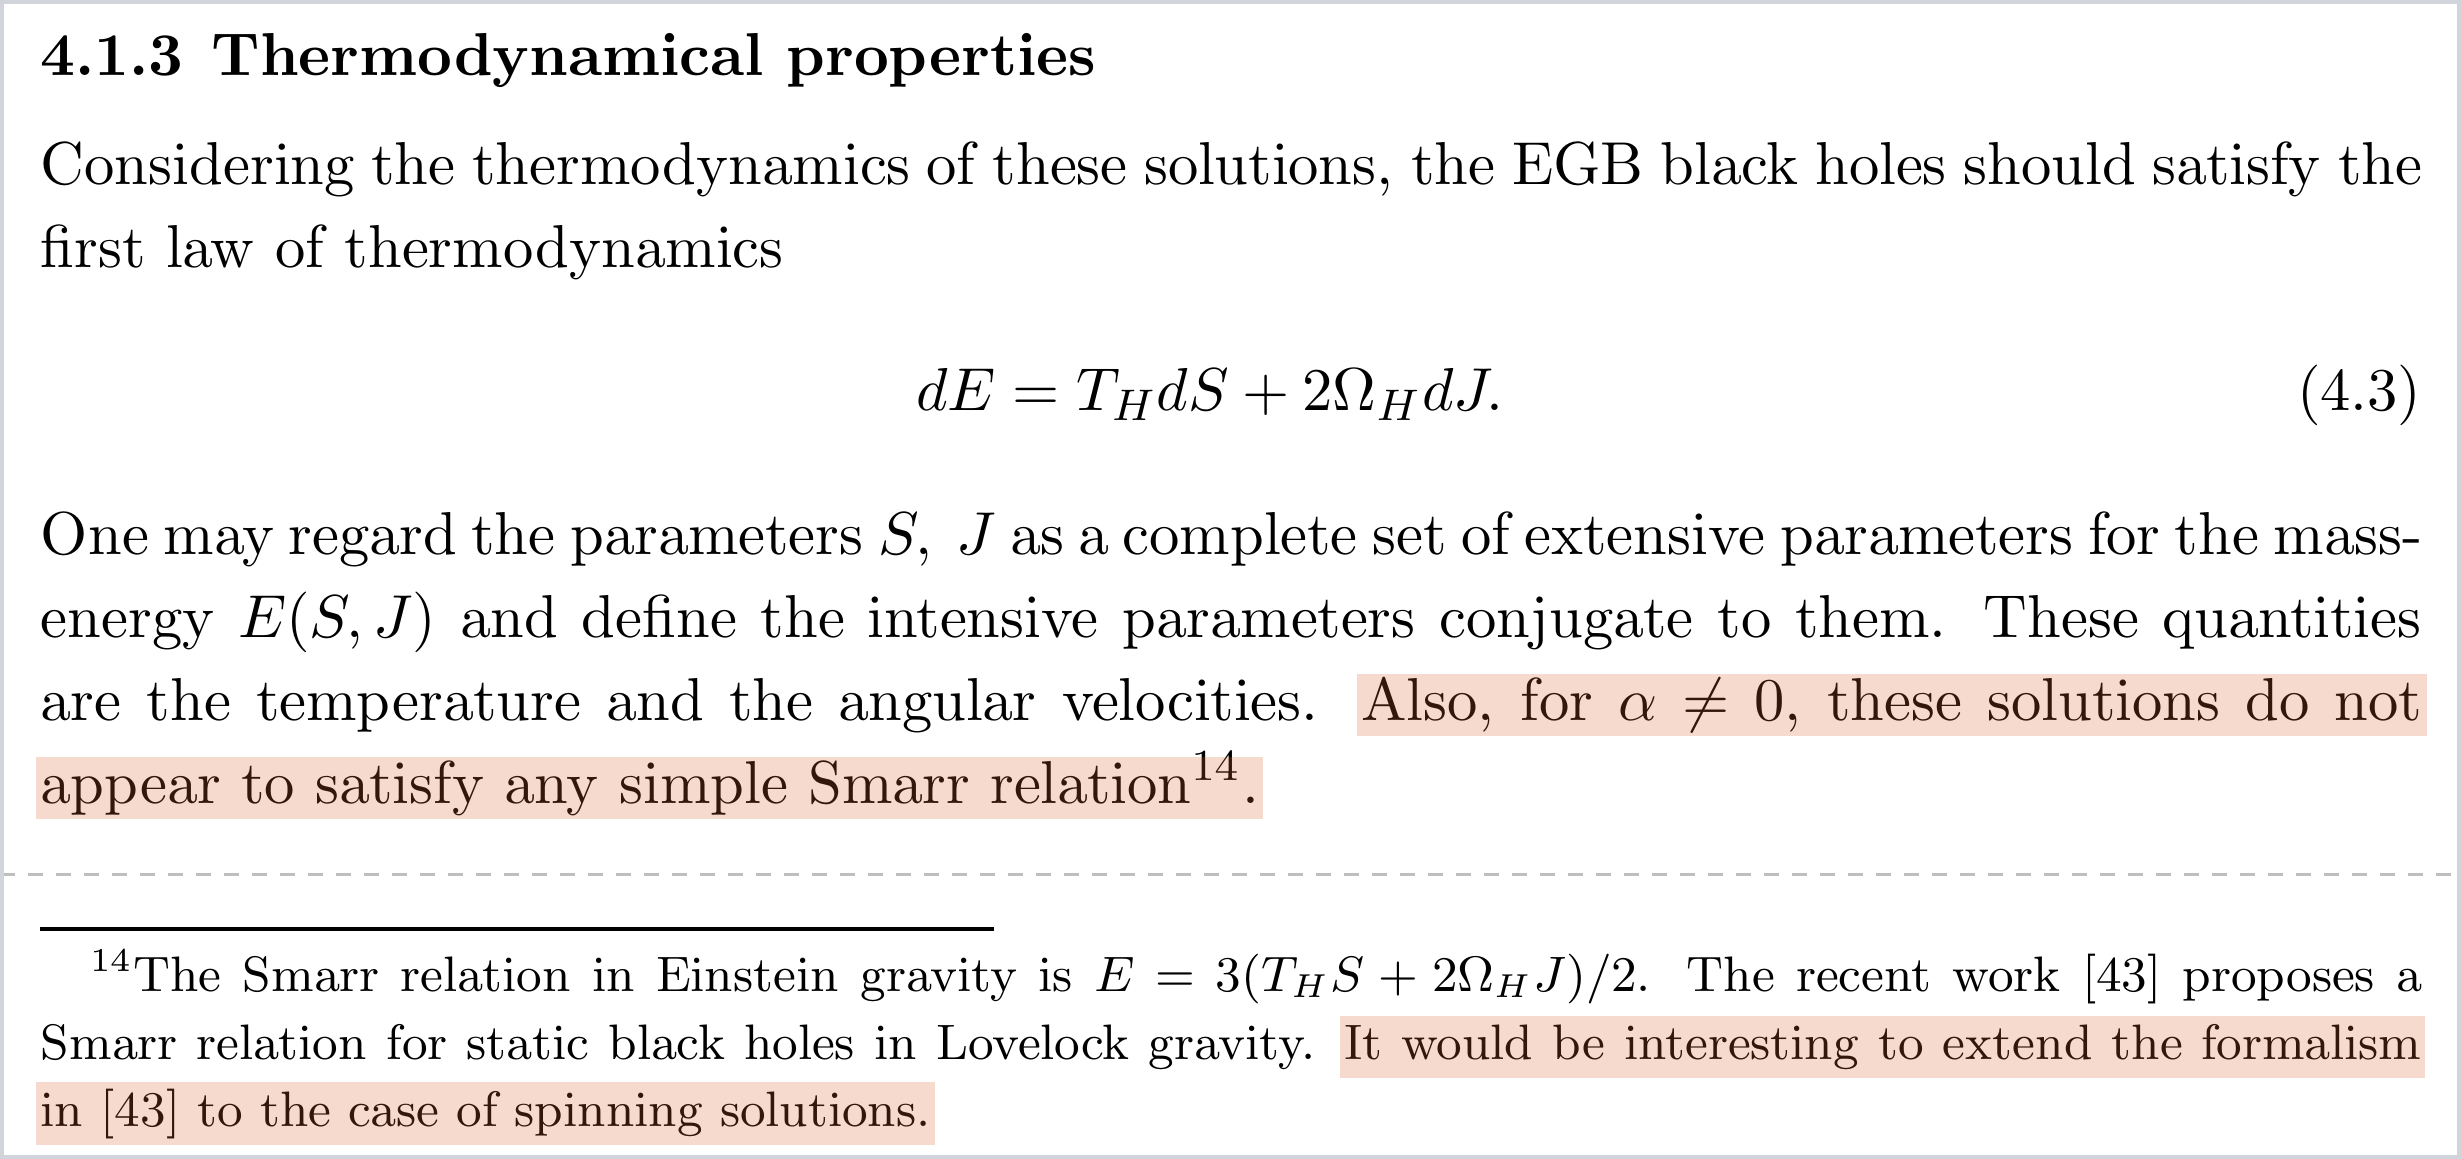
\includegraphics[width=\linewidth]{fig-smarr.png}\par\vspace{2pt}
{\tiny\color{muted}arXiv:1010.0860, \S4.1.3 and footnote 14.\par}
\vspace{4pt}
{\scriptsize Hito 6, $\alpha$ as a thermodynamic variable:\
$2M=3TS+6\Omega_HJ+2\alpha\Psi$\par}
\end{minipage}
\end{frame}

% ---------------------------------------------------------------- A5
\begin{frame}{A5 \textperiodcentered{} What it cost}
\centering
\begin{columns}[T,onlytextwidth]
\column{.25\textwidth}\centering\stat{36.8 h}{active agent time, 13 days}
\column{.25\textwidth}\centering\stat{1.42 billion}{tokens processed\\(99\% re-read context)}
\column{.25\textwidth}\centering\stat{5.9 million}{tokens written ($\approx$24 MB)}
\column{.25\textwidth}\centering\stat{79}{human prompts}
\end{columns}
\vspace{4pt}
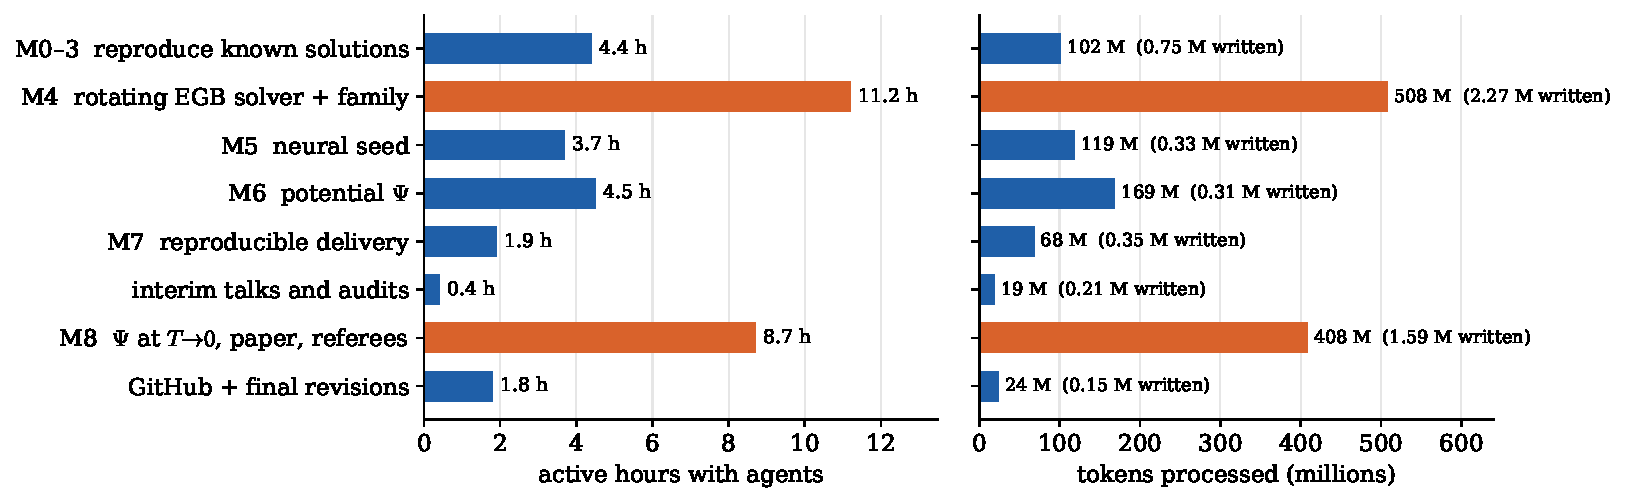
\includegraphics[width=.8\textwidth]{fig-cost.pdf}\\
\small The first \alert{new} object cost $5\times$ the tokens of reproducing everything known.\\[2pt]
\src{Not counted: human time, background numerical runs.}
\end{frame}

\end{document}
